\chapter{Circuit-Cocircuit algorithm}
\label{ch:algorithm}

\section{Abstract Circuit-Cocircuit meta-algorithm}

The problem of exhaustive generation of minimal edge cuts in \linebreak a graph can be generalized to the problem of exhaustive generation of cocircuits in a matroid.

\begin{defn}[Cycle matroid]
	\label{cycle_matroid}
	Given a connected graph $G$ its \textit{cycle matroid} is a matroid on the ground set $E(G)$ and its bases are the edges of the spanning trees of G. Moreover independent sets are the acylic subsets (forests) of G, circuits are the cycles of G and cocircuits are the minimal edge cuts of G.
\end{defn}

We will use the following folklore statement, see Oxley \cite{oxley2006matroid}.

\begin{prop}
	\label{prop_circuit-cocircuit}
	If $C$ is a~circuit and $X$ is a cocircuit in a matroid M, then ${\lvert C \cap X \rvert \neq 1}$.
\end{prop}

Using this proposition an algorithm with the following gist can be constructed. Start with any element of $M$ in $X$, find a circuit $C$, such that \linebreak ${\lvert C \cap X \rvert = 1}$ and then for each element $c \in C \setminus X$, add $c$ to $X$, verify there is a hyperplane in the complement of $X$ and continue recursively for as long as such circuits can be found.

\clearpage

\begin{algorithm}
	\caption{Abstract circuit-cocircuit meta-algorithm}
	\label{meta-algorithm}
\begin{algorithmic}[1]
	\Require Matroid $M = (E, \mathcal{B})$ and a cocircuit size bound $m \in \mathbb{N}$
	\Ensure All cocircuits of $M$ with size $\leq m$
	\State $B \leftarrow$ an arbitrary basis in $\mathcal{B}$
	\ForAll{$b \in B$}
		\State $X \leftarrow \{b\}$
		\State \Call{GenCocircuits}{$X$}
	\EndFor
	\Procedure{GenCocircuits}{$X$}
	\If{$E \setminus X$ contains no hyperlane of $M$ \textbf{or} $\lvert X \rvert > m$}
		\State \textsc{Abort}
	\EndIf
	\State Find any circuit $C \subseteq E$ such that $\lvert C \cap X \rvert = 1$
	\If{such $C$ doesn't exist}
		\State \textbf{return} $X$ \Comment{$X$ is a cocircuit}
	\Else
		\State $D \leftarrow C \setminus X$
		\ForAll{$c \in D$}
			\State \Call{GenCocircuits}{$X \cup \{c\}$}
		\EndFor
	\EndIf

	\EndProcedure
\end{algorithmic}
\end{algorithm}

\begin{thm}
	\label{meta_alg_correctness}
	Algorithm \ref{meta-algorithm} generates exactly all the cocircuits of size $\leq m$ in the matroid $M$.
\end{thm}

\begin{proof}
	First, we show that any set $X_0$ returned by the algorithm is a~cocircuit and $\lvert X_0 \rvert \leq m$. By the condition on line 7, the set $E \setminus X_0$ contains a~hyperplane $H$ of $M$ and $\lvert X_0 \rvert \leq m$. If $H = E \setminus X_0$ then we are done by Claim \ref{matroid_folklore}.c. Now suppose $H \neq E \setminus X_0$ and choose $e \in E \setminus (X_0 \cup H)$. According to Claim \ref{matroid_folklore}.b there is a basis $B_0 \subseteq H \cup \{e\}$. Choose $a \in X_0$ and let $C_0$ be the circuit contained in $B_0 \cup \{a\}$ according to Claim \ref{matroid_folklore}.a. Then $C_0 \cap X_0 = \{a\}$ contradicts the condition on line 11 and thus $H$ must be equal to $E \setminus X_0$.

	Second, we show that any cocircuit $X_1$, $\lvert X_1 \rvert \leq m$, is generated. Let ${Z_1 \subseteq X_1}$ be the largest subset of $X_1$ such that GenCocircuits($Z_1$) has been called. By Claim \ref{matroid_folklore}.d, $X_1 \cap B$ is nonempty for the basis $B$ selected on line $1$ and thus $Z_1$ is well-defined and non-empty.
	If ${Z_1 = X_1}$ then $X_1$ will be returned since it is a cocircuit and no circuit $C$ is found on line $10$. Suppose $Z_1 \neq X_1$ and choose $d \in X_1 \setminus Z_1$. By Claim \ref{matroid_folklore}.b there is a basis $B_1 \subseteq H_1 \cup \{d\}$ (where $H_1 := E \setminus X_1$ is a hyperplane of $M$). For any $b \in Z_1$, let $C_1$ be the circuit contained in $B_1 \cup \{b\}$ according to Claim \ref{matroid_folklore}.a. Consequently, there exists a~circuit $C$ to be found by the algorithm on line 10 (note that it may be $C \neq C_1$). Since $\lvert C \cap X_1 \rvert \neq 1$, there exists $d' \in C \cap X_1$ such that $d'\not\in Z_1$, and \textsc{GenCocircuits}($Z_1 \cup \{d'\}$) is eventually called, contradicting the maximality of $Z_1$.
\end{proof}

\begin{cor}
	\label{cor_circuit_subset}
	Algorithm \ref{meta-algorithm} remains correct even if line 14 sets $D$ to be a subset of $C \setminus X$, such that $D$ is guaranteed to intersect every cocircuit $X_1 \supseteq X$ in $M$.
\end{cor}

\begin{proof}
	TODO
\end{proof}

\section{$2$-way cuts in a graph}

We present details of implementing the meta-algorithm to generate $2$-way cuts in a given graph.

We introduce a colouring of the graph (in the sense of labeling) to help us decide the hyperplane existence question on line 7. During the progress of the algorithm some edge $e$ is chosen to be added to $X$ and the algorithm continues to call \textsc{GenCocircuits}. Before this call we colour one end of $e$ red and the other blue. When adding the first edge $e = \{u ,v\}$ to $X$ it is arbitrary whether $u$ is coloured red and $v$ blue (or vice versa). The situation with the next edges added to $X$ is described below. This colouring has to be consistent among edges sharing a vertex.

Let $V(X) = V_r \cup V_b$ and call $V_r$ the red vertices of $X$ and $V_b$ the blue vertices of $X$. We maintain a red tree $T_r$ interconnecting $V_r$. Call ${T_b \subseteq (G \setminus T_r \setminus X)}$ the blue tree interconnecting $V_b$. It will turn out that it is not necessary to store this tree explicitly in a variable.

We add to $T_r$ only those edges $e$ for which it is guaranteed that \textsc{GenCocircuits} is called with $X \cup \{e\}$. We do not remove elements from $T_r$ (within recursive calls) while elements may be removed from $T_b$ and added to $X$. This shows that $T_r$ and $T_b$ are not treated symmetrically. In the end we want to have a cut $X$ separating the graph into two connected components: $T_r$ in one component, $T_b$ in the other. It follows that $V(T_r) \cap V(T_b) = \varnothing$ and $V_r \subseteq V(T_r)$, $V_b \subseteq V(T_b)$.


TODO: Refine this lemma and its proof.

\begin{lem}
	\label{lem:hyperplane_existence}
	Let $G$ be a~connected graph, $M = (E, \mathcal{B})$ its corresponding cycle matroid and $Y \subseteq E(G)$. $E \setminus Y$ contains a hyperplane if, and only if, the vertices of each edge in $Y$ can be coloured red and blue such that this colouring is consistent among the edges in $Y$ and such that the vertices of each colour can be connected by a tree in $G \sm Y$.
\end{lem}


\begin{proof}
	$(=>)$
	If $E \sm Y$ contains a hyperplane, then there exists a~cocircuit $X \supseteq Y$ by Claim \ref{matroid_folklore}.c. By Definition \ref{cycle_matroid} $X$ is a bond in $G$ and $G \sm X$ has two connected components, as more components would contradict the minimality of $X$. Colouring one of this components red and the other blue yields finishes the argument.

	$(<=)$ Given are two trees, one coloured red and the other blue. Start in one vertex of the red tree and traverse graph $G$ without crossing the to-be generated bond $X \supseteq Y$. Repeat this procedure in the blue tree. This determines some bond $X$, therefore a cocircuit in $M$ and thus by Claim \ref{matroid_folklore}.c a~hyperplane $E \sm X$. Since $Y \subseteq X$ then $E \sm Y$ contains a hyperplane.

\end{proof}


\subsection*{Modifying Algorithm \ref{meta-algorithm} to generate $2$-bonds of a graph}

\begin{rec}
	Let $M$ be the cycle matroid of graph $G$. The bases, circuits, cocircuits of $M$ are the sets of edges of the spanning trees, cycles and bonds in $G$.
\end{rec}

\begin{itemize}
	\item On line 1 choose an arbitrary spanning tree of $G$.

	\item On line 3 the existence of a~hyperplane can be easily decided with use of Lemma \ref{lem:hyperplane_existence} and the previously defined colouring. $E \setminus X$ contains a hyperplane of $M$ if, and only if, $T_r$ and $T_b$ are both connected subgraphs of $G$.

	\item Choose $D$ to be the shortest path in $G \setminus X$ between a vertex from $V(T_r)$ and a vertex from $V_b$. For every such $D$, it holds that $D \cap E(T_r) = \varnothing$ and there exists a cycle $C \subseteq D \cup E(T_r) \cup X$ in $G$ with $\lvert C \cap X \rvert = 1$.

\end{itemize}

TODO: Prove there exists the cycle $C$ in the last item

First two modifications are possible from the definition of cycle matroid. For the third modification we have to show that the path $D$ is chosen such that it satisfies the requirements from corollary \ref{cor_circuit_subset}. It follows from an easy induction argument:

In the base case, that is before choosing the first circuit, the modification does not affect anything since $T_r = \varnothing$ -- all the subsets of the to-be-generated $2$-bonds are chosen. Now consider an arbitrary recursive call to \textsc{GenCocircuits}. By the induction hypothesis the algorithm has not missed any subset of some $2$-bond yet and by the colouring scheme above we add to $T_r$ only those edges $e$ for which the algorithm guarantees it has called \textsc{GenCocircuits}$(X \cup \{e\})$.

\section{$k$-way cuts in graph}

The above described implementation of Algorithm \ref{meta-algorithm} generates the $2$-bonds of some connected graph $G$. Now consider $G' = G \setminus Y$, where $Y$ is a $2$-bond of $G$. $G'$ has two connected components and we can apply the algorithm again to each of them to generate the $2$-bonds of the components. It can be proved that the union of $Y$ and any $2$-bond of $G'$ is a $3$-bond of $G$. Such a recursive application of the algorithm can be used to generate all $k$-bonds for some given $k \geq 0$. To formalize this \textit{stepwise} approach and to set it up within the scheme of Meta-algorithm \ref{meta-algorithm}, we start with the definition of $k$-way cycle matroid.

\begin{defn}[$k$-way cycle matroid]
	\label{kway_cycle_matroid}
	Let $G$ be a graph on less than $k \geq 2$ connected components. The \textit{$k$-way cycle matroid} of $G$ is a matroid on the ground set $E(G)$, such that its bases are the edge sets of the spanning forests of $G$ that consist of $k-1$ trees.

	The bases, circuits, cocircuits and hyperplanes of the $k$-way cycle matroid are also called the $k$-way bases, circuits, cocircuits, hyperplanes of $G$.
\end{defn}

From the definition above we may conclude the following claim.

\begin{claim}
	\label{circuit_types}
	Let $G$ be a graph consisting of less than $k \geq 2$ connected components.
	The $k$-way cocircuits of $G$ are the $k$-bonds of $G$. The $k$-way circuits of $G$ are of two types, \textit{type-C} and \textit{type-F}.

	\begin{enumerate}
		\item Type-C circuits are the graph cycles in $G$.
		\item Type-F circuits, also called \textit{spanning circuits}, for $k \geq 3$, are the spanning forests of $G$ that are formed by $k-2$ trees.
	\end{enumerate}
\end{claim}

Before defining the stepwise circuit-cocircuit implementation we first need to introduce the following technical term. The \textit{level $i$ of recursion} in Algorithm \ref{meta-algorithm} is the number of calls to the procedure \textsc{GenCocircuits} currently being processed (on the \textit{call stack}).

\begin{defn}[Stepwise circuit-cocircuit implementation scheme]
	\label{defn:stepwise_scheme}

	We call an implementation of Algorithm \ref{meta-algorithm} \textit{stepwise} if, for every set $X = X_0$, $\lvert X_0 \rvert = l$, generated by the algorithm,

	\begin{enumerate}
		\item $X_0$ is an ordered sequence $(c_1, c_2,\ldots,c_l)$, where $c_i$ has been \linebreak added to $X_0$ at the level $i-1$ of recursion,
		\item there exists a mapping $s : \{1,2,\ldots,k\} \rightarrow \{0,1,\ldots,l\}$ such that $s(1) = 0$, $s(k) = l$ and, for each $j \in \{2,\ldots,k-1\}$, the set $\{c_1,\ldots,c_{s(j)}\} \subsetneq X_0$ forms a $j$-bond in $G$.
	\end{enumerate}

	\noindent For $j$, $1 \leq j < k$, we call the \textit{$j$-th stage of the algorithm} the steps the algorithm does at the levels $s(j), s(j) + 1,\ldots, s(j+1)-1$ of recursion. The algorithm selects elements $c_{s(j)+1},\ldots,c_{s(j+1)}$ in the $j$-th stage.

\end{defn}

\begin{defn}[Stepwise partition]
	\label{defn:stepwise_partition}

	Let $Z$ be a $k$-bond. For $1 \leq j < k$, let $Z^{j} = \{c_{s(j)+1},\ldots,c_{s(j+1)}\}$. An ordered partition $(Z^1, \ldots, Z^{k-1})$ of $X_0$ is called a stepwise partition if there exists a stepwise implementation (confer Definition \ref{defn:stepwise_scheme}) of Algorithm \ref{meta-algorithm}, such that the elements of $Z^j$ are added to $X$ in its $j$-th stage.

\end{defn}

\begin{rem}
	There is a one to one correspondence between the stepwise partition and the mapping $s$.
\end{rem}

\begin{rem}
	Not every ordering of $\{Z^1, \ldots, Z^{k-1}\}$ is a valid stepwise partition. On the other hand, by Lemma \ref{stepwise_is_welldefined}, there exists a valid stepwise partition for each $k$-bond.
\end{rem}

The following lemma asserts that the $k$-bonds can be generated by a stepwise implementation of the Circuit-Cocircuit algorithm.

\begin{lem}
	\label{stepwise_is_welldefined}
	Let $G$ be a connected graph and $X \subseteq E(G)$ a $k$-bond, $k \geq 2$.
	For any $i$-bond $Z \subset X$ of $G$, $i < k$, there exists an $(i+1)$-bond $Y$ of $G$ such that $X \supseteq Y \supset Z$.
\end{lem}

\begin{proof}
	TODO: Update proof.

	Let $G'' = G \setminus X$. Consider a set of edges $A \subseteq X$ such that $G'' \cup A$ has $(i+1)$ connected components. If $A$ is maximal such set, then there exists some $(i+1)$-bond $Y = X \setminus A$.

	Now let $G' = G \setminus Y$. Consider a set $B \subseteq Y$ such that $G' \cup B$ has $i$~connected components. Such $B$ exists, because $Y$ is a~minimal $(i+1)$-way cut, thus $G' \cup \{f\}$ has $i$-connected components for some $f~\in~Y$. If $B$ is maximal set such that $G' \cup B$ has $i$ connected components, then there is some $i$-bond $Z = Y \setminus B = X \setminus (A \cup B)$.

	In the base case this construction is clearly possible and the \linebreak lemma follows by induction.
\end{proof}

With Theorem \ref{meta_alg_correctness} and Lemma \ref{stepwise_is_welldefined} we can easily conclude:

\begin{thm}
	\label{thm:stepwise_impl_correctness}
	For any given graph $G$ a stepwise implementation of Algorithm \ref{meta-algorithm} can be used to generate all the $k$-bonds in $G$.
\end{thm}


\noindent We will also use the following two technical lemmas.

\begin{lem}
	\label{stepwise_2bond}
	Let $G$ be a connected graph and $X \subseteq E(G)$ any $k$-bond, and for~$j$,~$1 \leq j \leq k$, denote by $X^j$ the set $\{c_1,\ldots,c_{s(j)}\}$ and by $G^j$ the graph $G \setminus X^{j}$. For $j$, $1 \leq j < k$, there is a connected component $G_0^j$ of $G^j$ such that $Z^j = X^{j+1} \setminus X^{j} \subseteq E(G_0^j)$ and $Z^j$ is a $2$-bond in $G_0^j$.
\end{lem}

\begin{proof}
	The set $B$ from the proof of Lemma \ref{stepwise_is_welldefined} is a $2$-bond.
\end{proof}


\begin{lem}
	\label{lem:kway_circuit_types}
	For each stage $j$, $1 < j < k$, of a stepwise implementation of the Circuit-Cocircuit Meta-algorithm \ref{meta-algorithm} respecting the Definition \ref{defn:stepwise_scheme} holds the following,

	\begin{enumerate}[label=\alph*.]
		\item the set $C$ chosen on line 10 at the level $s(j)$ has to be a type-F (spanning) circuit,
		\item at the levels $i$, $s(j)+1 \leq i < s(j+1)$ of recursion, the set $C$ can always be chosen as a type-C circuit.
	\end{enumerate}
\end{lem}

\begin{proof}[Proof (\ref{lem:kway_circuit_types}.a)]
	In each stage $j$, the first edge the algoritm selects is $c_{s(j)+1}$ from $C$ which is a $k$-way circuit in $G$. Since the set $\{c_1,\ldots,c_{s(j)}\}$ forms a $j$-bond in $G$, the value of $C$ at the level $s(j)$ cannot be a type-C circuit and thus it has to be a type-F circuit by Claim \ref{circuit_types}.
\end{proof}

\begin{proof}[Proof (\ref{lem:kway_circuit_types}.b)]
	By its construction the set $B$ in proof of Lemma \ref{stepwise_is_welldefined} has exactly one edge, call it $f$, from some type-F circuit and each edge $e \in (B \setminus \{f\})$ lies in a type-C circuit together with $f$.
\end{proof}

\subsection*{Extending a $j$-bond to $(j+1)$-bonds}

To modify the original algorithm to fit into the scheme for generating $k$-bonds we solve the problem of extending a given $j$-bond $Y$ into a set of $(j+1)$-bonds, each of them a superset of $Y$.

\begin{algorithm}
	\caption{One stage of stepwise implementation}
	\label{algorithm-one_stage}
\begin{algorithmic}[1]
	\Require A connected graph $G$, parameters $j, k, m \in \mathbb{N}, j < k, m \geq 1$, and a $j$-bond $Y_1 \subseteq E(G)$
	\Ensure A collection of $(j+1)$-bonds such that for each $k$-bond $Y$, $Y_1 \subseteq Y \subseteq E(G)$, $\lvert Y \rvert \leq m$, some subset of $Y$ is among the generated $(j+1)$-bonds
	\If{$j=1$} \Comment{$Y_1 = \varnothing$, select a $k$-way basis}
		\State $F \leftarrow$ an arb. spanning forest of $k-1$ trees
		\Else \Comment{$Y_1 \neq \varnothing$, select a type-F circuit}
		\State $F \leftarrow$ an arb. spanning forest of $k-2$ trees and ${\lvert F \cap Y_1 \rvert = 1}$
	\EndIf
	\ForAll{$d = \{u, v\} \in F \setminus Y_1$}
		\State \Call{GenStage}{$j, Y_1, X = \{d\}, V_r = \{u\}, V_b = \{v\}, T_r = \{u\}$}
	\EndFor

	\Procedure{GenStage}{$j, Y, X, V_r, V_b, T_r$}
	\State Let $G_1 \subseteq G$ be the component of $G \setminus Y$ containing $X$
	\If{$\lvert Y \cup X \rvert > m - k + j + 1$}
		\State \textbf{return;}
	\EndIf
	\If{there does not exist a connected subgraph \\
		\qquad \enspace $T_b \subseteq (G_1 \sm V(T_r)) \sm X$ such that $V_b \subsetneq V(T_b)$}
		\State \textbf{return;}
	\EndIf
	\State $P \leftarrow$ a (short) $V(T_r){-}V_b$ path $P \subseteq G_1$

	\If{such $P$ does not exist}
		\State \textbf{return} $Y \cup X$ \Comment{$Y \cup X$ is a $j+1$-bond}
	\Else
		\ForAll{$c \in P$}
			\State Let $u$ be the vertex in $c = \{u,v\}$ which is closer to $T_r$
			\State Let $P_u$ be the component of $P - c$ which contains $u$
			\State \Call{GenStage}{$j, Y, X \cup \{c\}, V_r \cup \{u\}, V_b \cup \{v\}, T_r \cup P_u$}
		\EndFor
	\EndIf

	\EndProcedure
\end{algorithmic}
\end{algorithm}

\clearpage

TODO: Fix this theorem and its proof.

\begin{thm}
	Let $G$ be a graph, $j,k,m$ natural numbers such that $j < k, m \geq 1$ and $Y_1 \subseteq E(G)$ a $j$-bond in $G$. Algorithm \ref{algorithm-one_stage} generates a set $\mathcal{S}$ of $(j+1)$-bonds such that for each $k$-bond $Y$, $Y_1 \subseteq Y \subseteq E(G)$, $\lvert Y \rvert \leq m$, some subset of $Y$ is among the generated $(j+1)$-bonds in $\mathcal{S}$.
\end{thm}

\begin{proof}
	It follows from Lemma \ref{stepwise_is_welldefined}, that for the given $Y_1$ and each $k$-bond $Y$ such that $Y_1 \subseteq Y$, there is $Y_2 \in \mathcal{S}$ such that $Y_1 \subsetneq Y_2 \subseteq Y$. We have to show that the algorithm generates this $Y_2$.

	If $j = 1$, the first edge $c_1 = c_{s(1)+1} \in Y_2 \setminus Y_1$ has to be chosen from a $k$-way basis and the algorithm does this by line 2. If $j > 1$, by Lemma \ref{lem:kway_circuit_types}.a, the edge $c_{s(j)+1} \in Y_2 \setminus Y_1$ has to be chosen from a \break type-F circuit -- the algorithm does this choice on line 4.

 For both $j = 1$ and $j > 1$, when choosing the remaining edges of $Y_2 \setminus Y_1$ in the steps $s(j) + 1, \ldots, s(j+1)-1$, the algorithm selects them from a type-C circuit, which is possible by Lemma \ref{lem:kway_circuit_types}.b.

%	Next we have to show that each edge is considered into X. Suppose the algorithm does not call \textsc{GenCocircuits}$(X \cup \{e\})$ for some edge $e \in Y$. This means that the choice of $C$ containing this $e$ was not made, contradicting the convergence of the algorithm.

 It remains to show that all $Y_2 \in \mathcal{S}$ such that $Y_1 \subsetneq Y_2 \subseteq Y$ with a certain $X_1 \subseteq Y_2 \setminus Y_1$ satisfy the size bound $\lvert Y_1 \cup X_1 \rvert \leq m - k + j + 1$. Suppose $\lvert Y_1 \cup X_1 \rvert > m - k + j + 1$. Thus in the next $k - j - 1$ stages the algorithm has to select less than $k - j - 1$ edges in the remaining steps to satisfy $\lvert Y \rvert \leq m$, contradicting our assumption that $Y$ is a $k$-bond.
\end{proof}


\chapter{Canonical generation}
\label{ch:canonical}

Algorithm \ref{algorithm-one_stage} generates many permutations of the same set. This becomes a problem especially when computing $k$-bonds for $k \geq 2$ because the algorithm is then called for each of the different permutations and generates the same $k$-bond more than once.

To reduce multiple generation of $k$-bonds we implement a technique of \textit{canonical generation}. McKay in \cite{mckay_isom} both presents an overview of various approaches to canonical generation and describes in detail the technique of \textit{generation by canonical construction path} which is the basis for our approach. We start by outlining the general idea.

\subsection*{Generation by canonical construction path}

Say we are generating some \textit{labeled} objects $\vec X$ and there is an equivalence relation $\simeq$ on the set of these objects. We apply generation by canonical construction path to generate only one object from each equivalence class of $\simeq$.

For each equivalence class $\mathcal{C}$ of $\simeq$ we (carefully) choose in advance a unique \textit{canonical representative}. We denote the canonical representative $\mcan(\vec X)$ for some $\vec X \in \mathcal{C}$.

At each iteration of the generating procedure we start with a partial solution $\vec Y$ and we \textit{check} whether this augmentation of $\vec Y$ is a prefix of $\mcan(\vec X)$, where $\vec X$ is some complete solution made from $\vec Y$. Note that this check is allowed to have false positives (that is allow augmentation which does not lead to the canonical solution) but no false negatives.

At the end of the generating procedure there is a complete solution \linebreak ${\vec X = \mcan(\vec{X}) }$ and the algorithm outputs it.

\sectionline

The definition of $\mcan()$ has to be compatible with the original generating routine so it is feasible to test $X$ against this definition often in the algorithm and so it does not miss any solution. On the other hand one wants to choose $\mcan()$ such that it prunes the search tree of the generating procedure\footnote{A tree where the root marks the start of the algortihm, inner nodes contain partial solutions and leafs mark the end of a branch of computation} to the utmost possible measure.

\clearpage

\section{Canonical generation of $k$-bonds}

We apply the idea of generation by canonical construction path to Algorithm \ref{algorithm-one_stage}. Before continuing we suggest to recall the Definition \ref{defn:stepwise_partition}.

Let $G$ be a connected graph and $X \subseteq E(G)$ a $k$-bond. For each \break $j \in \{1, \ldots, k\}$, denote by $G^j$ the set $G \setminus \{c_{1}, \ldots, c_{s(j)}\}$, and by $G^j_0$ the connected component of $G^j$ such that $Z^j \subseteq E(G^j_0)$.

TODO: Recall $Z^j$?

\begin{defn}[Canonical form of a stepwise partition]
	\label{can}

	Let $G$ be a connected graph, $X \subseteq E(G)$ a $k$-bond with $\lvert X \rvert = l$, $\mathcal{Z}$ a stepwise partition of $X$ and $s$ a mapping dependent on $X$ (confer Definition \ref{defn:stepwise_scheme}). Furthermore let
	$\iota : E(G) \rightarrow \{1,\ldots,\lvert E(G) \rvert\}, \> \nu : V(G) \rightarrow \{1,\ldots,\lvert V(G) \rvert\}$ be arbitrary bijections (indexing the edges and vertices) and let $\lambda : E(G) \rightarrow \mathbb{N}$ be an arbitrary mapping. The~\textit{canonical form} of $\mathcal{Z}$, $can(\mathcal{Z}) = (c_1, c_2,\ldots, c_l)$, is a permutation of $X$ which satisfies the following, for each $j \in \{1,\ldots,k-1\}$:

	\begin{enumerate}[label=\alph*.]
		\item Let $u,v$ be the ends of $c_{s(j)+1} \in Z^j$. The vertices of edges in $Z_j$ can be bipartitioned as $V(Z^j) = V^j_r \dot\bigcup V^j_b$, such that each edge of $Z^j$ has one of its ends in $V_b^j$ and the other in $V_r^j$. Moreover $u \in V_r^j$ if and only if $\nu(u) < \nu(v)$.

		\item The edge $c_{s(j)+1}$ satisfies ${\iota(c_{s(j)+1}) = \min\{ \iota(c_i) : s(j) < i \leq s(k) \}}$

	\item For each $i \in \{s(j) + 2,\ldots, s(j+1)\}$,
		let $P_{u,v} \subseteq G^j_0$ be a certain path with ends $u,v$,
		let $c_i$ be the edge of $E(P) \cap Z^j$ closest to the end $u$ in $P$ and let
		$Y_{ji} = \{c_{s(j)+1}, \ldots, c_i\} \subseteq Z^j$.

		Define $P_{u,v} \subseteq G_0^j \setminus Y_{ji}$ to be the \textit{unique shortest path}, such that among all $V_r(Y){-}V_b(Y)$ paths in $G^j_0 \setminus Y_{ji}$, it lexicographically minimizes the triplet
	$(\lvert E(P) \rvert, \mlen_\lambda(P), \vec{\iota}(P) )$, where $\mlen_\lambda(P) = \sum_{e \in E(P)} \lambda(e)$ and $\vec{\iota}(P) = (\iota(e_1), \iota(e_2),\ldots, \iota(e_{\lvert E(P) \rvert}))$.

	\end{enumerate}

\end{defn}


\noindent
\begin{note}
The first point of the above definition uses Lemma \ref{stepwise_2bond}.
\end{note}

\clearpage %%%%%%%%%%%%

\noindent
To shorten our notation we introduce $\mu$ and $\tau$ as follows.

%%
% I also liked the definition of \tau using c_{s(j)+1}, where j is the largest index added to X.
%%

\begin{defn}
	Let $\iota$ be an arbitrary bijection (confer Definition \ref{can}), $Z$ be a $k$-bond with stepwise partition $(Z^1,\ldots,Z^{k-1})$, $s$ be a mapping as in Definition \ref{defn:stepwise_scheme} and $1 \leq j \leq k - 1$.

\[
	\mu(Z^j) \stackrel{\text{def}}{=} \min\{ \iota(c) : \in Z^j \}
\]

\medskip

\noindent
Now let $Y$ be a prefix of $X$ with partition $(Z^1,\ldots, Z^h)$, $h < k$.

	\[
		\tau(Y) \stackrel{\text{def}}{=}
		\begin{cases}
			\hfill -\infty    		 \hfill & \text{if $Y = \varnothing$} \\
			\hfill \mu(Z^h) \hfill & \text{otherwise} \\
		\end{cases}
	\]

\end{defn}


\begin{defn}[Canonical form of a bond]
	\label{defn:can_bond}

	Let $G$ be a graph and $X \subseteq E(G)$ be a $k$-bond. Define $can(X)$ to be the canonical form of some stepwise partition $(Z^1,\ldots,Z^{k-1})$ of $X$, such that $\mu(Z^1) < \mu(Z^2) < \ldots < \mu(Z^{k-1})$.
\end{defn}


\begin{lem}
	\label{lem:every_kbond_has_can}
	For every $k$-bond $X$ there exists a canonical form of $X$.
\end{lem}

\begin{proof}
	We proceed by induction on the number of stages. First we show that the edge $c_1 = c_{s(1)+1} \in \vec{X}$ satisfying (by Definition \ref{can}) $\iota(c_{s(1)+1}) = min\{ \iota(c_i) : s(1) < i \leq s(k) \}$, lies in the $\iota$-minimum $k$-way basis, that is the $\iota$-minimum spanning forest $F \subseteq G$ consisting of $k-1$ trees.

	For a contradiction suppose that $c_{s(1)+1}$ does not lie in $F$. Because $\vec X$ is a cocircuit of $G$, it intersects every basis of $G$ including the $\iota$-minimal one $F$, by Proposition \ref{matroid_folklore}. Say there is an element $e$ in the intersection of $\vec X$ with $F$. Then $F \cup \{c_{s(1)+1}\}$ contains a circuit through $e$. The set $F' = F \cup \{c_{s(1)+1}\} \setminus \{e\}$ is a basis such that

\[
	\sum_{e \in F'} \iota(e) < \sum_{e \in F} \iota(e)
\]

This contradicts the assumption that $F$ is a minimum basis.

	By lemmas \ref{circuit_types} and \ref{stepwise_is_welldefined} the rest of the edges of this first stage can be selected as a type-C circuit. For each edge the algorithm selects the unique path (satisfying Definition \ref{can}) which is contained in an implicit type-C circuit (confer Corollary \ref{cor_circuit_subset}). This finishes the first stage.

	For the induction step consider the $j$-th stage and a $j$-bond $Y \subseteq \vec X$. We want to show that the edge $c_{s(j)+1} \in \vec X$ lies in the $\iota$-minimum type-F circuit, that is a $\iota$-minimum spanning forest $F$ on $k-2$ trees. Since $\lvert F \cap Y \rvert = 1$, it suffices to show that the edge $c_{s(j)+1}$ lies on a $\iota$-minimum spanning forest $S = F \sm Y$ on $k-1$ trees (again a $k$-way basis) such that and $Y \cap S = \varnothing$. To prove this we provide a very similar argument as in the base case:

	For a contradiction suppose that $c_{s(j)+1}$ does not lie in $S$. Because $\vec X$ is a cocircuit of $G$, it intersects every basis of $G$. Say there is an element $e$ in the intersection of $\vec X$ with $S$. Then $S \cup \{c_{s(1)+1}\}$ contains a circuit through $e$. The set $S' = S \cup \{c_{s(j)+1}\} \setminus \{e\}$ is a basis contradicting our assumption that $S$ is minimum.


	The rest of the edges of this $j$-th stage is chosen in the same way as in the first stage. This finishes the induction step.
\end{proof}

\begin{exmp*}
	The canonical form of $X$ is not unique.
	Let $k = 3$, $m = 3$. In stage 1 the algorithm generates bonds $(0,1)$ and $(0,2)$. In stage 2 bond $(0,1)$ is extended to $(0,1,2)$ and bond $(0,2)$ is extended to $(0,2,1)$.

	\begin{center}
		% 
% dot2tex --autosize tmp/graph9.tmp --prog neato --figonly
%

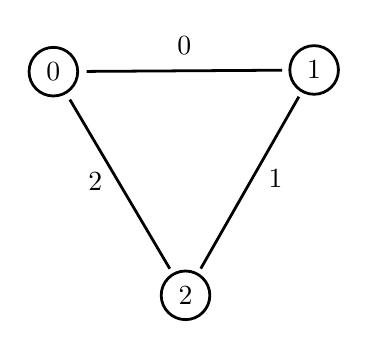
\begin{tikzpicture}[>=latex,line join=bevel,real/.append style={circle, draw=black} ]
  \pgfsetlinewidth{1bp}
%%
\pgfsetcolor{black}
  % Edge: 0 -- 1
  \draw [] (-35.2bp,26.724bp) .. controls (-15.446bp,26.841bp) and (15.392bp,27.043bp)  .. (35.2bp,27.159bp);
  \definecolor{strokecol}{rgb}{0.0,0.0,0.0};
  \pgfsetstrokecolor{strokecol}
  \draw (0bp,35.941bp) node {0};
  % Edge: 2 -- 0
  \draw [] (-5.2199bp,-44.329bp) .. controls (-14.277bp,-29bp) and (-31.973bp,0.95243bp)  .. (-41.211bp,16.588bp);
  \draw (-32.1bp,-12.8705bp) node {2};
  % Edge: 1 -- 2
  \draw [] (41.229bp,17.623bp) .. controls (32.319bp,2.0092bp) and (14.815bp,-28.662bp)  .. (5.9095bp,-44.269bp);
  \draw (32.8bp,-12bp) node {1};
  % Node: 1
\begin{scope}
  \definecolor{strokecol}{rgb}{0.0,0.0,0.0};
  \pgfsetstrokecolor{strokecol}
  \draw (46.722bp,27.249bp) node [real] {1};
\end{scope}
  % Node: 0
\begin{scope}
  \definecolor{strokecol}{rgb}{0.0,0.0,0.0};
  \pgfsetstrokecolor{strokecol}
  \draw (-47.146bp,26.633bp) node [real] {0};
\end{scope}
  % Node: 2
\begin{scope}
  \definecolor{strokecol}{rgb}{0.0,0.0,0.0};
  \pgfsetstrokecolor{strokecol}
  \draw (0.42374bp,-53.881bp) node [real] {2};
\end{scope}
%
\end{tikzpicture}


	\end{center}

\vspace{-0.5cm}
\end{exmp*}

\subsection*{Achieving the canonical generation within Algorithm \ref{algorithm-one_stage}}

\begin{itemize}
	\item At the beginning of each stage the edge $c$ which is being added to $X$ has to satisfy $\iota(c) > \tau(Y)$. Note that as a result the spanning forest $F$ has to be recomputed at the beginning of each stage

	\item Within each stage, after the first edge has been chosen then all the edges $c'$ being added to $X$ have to satisfy $\iota(c') > \tau(Y)$

	\item The path $P$ is chosen on line 18 such that it satisfies the condition of Definition \ref{can}.c.

	\item The choice of edge $c \in E(P) \cap Z^j$, such that it is the edge in $E(P) \cap Z^j$ closest to $T_r$, is embedded in the algorithm by iterating through the edges of $P$ \textit{in order} ("red $\rightarrow$ blue")

\end{itemize}

\clearpage

\begin{algorithm}
	\caption{One canonical stage of stepwise implementation}
	\label{algorithm-can_one_step}
\begin{algorithmic}[1]
	\Require A connected graph $G$, parameters $j,\, k,\, m \in \mathbb{N},\, j < k,\, m \geq 1$ and a~$j$-bond $Y_1 \subseteq E(G)$
	\Ensure A collection of $(j+1)$-bonds as in Algorithm \ref{algorithm-one_stage}), such that each one is in the unique canonical form extending $Y_1$

	\If{$j=1$}
		\State $F \leftarrow$ a $\iota$-minimum spanning forest of $k-1$ trees
		\Else
		\State $F \leftarrow$ a $\iota$-minimum spanning forest of $k-2$ trees, $\lvert F \cap Y_1 \rvert = 1$
	\EndIf

	\ForAll{$d = \{u, v\} \in F \setminus \{e \in E(G) \mid \iota(e) \leq \tau(Y_1) \} $}
		\State \textbf{if} $ \, \nu(v) < \nu(u)$ \textbf{then}  $u,v \leftarrow v, u \,$ \textbf{fi}
		\State \Call{GenStage}{$j, Y_1, X = \{d\}, V_r = \{u\}, V_b = \{v\}, T_r = \{u\}$}
	\EndFor

	\Procedure{GenStage}{$j, Y, X, V_r, V_b, T_r$}
	\State Let $G_1 \subseteq G$ be the conn. component of $G \setminus Y$ containing $X$
	\If{$\lvert Y \cup X \rvert > m - k + j + 1$}
		\State \textbf{return;}
	\EndIf
	\If{there does not exist a connected subgraph \\ \qquad \enspace  $T_b \subseteq (G_1 \setminus V(T_r)) \setminus X$ such that $V_b \subseteq V(T_b)$}
		\State \textbf{return;}
	\EndIf
	\State $P' \leftarrow$ a path $P' \subseteq G_1$ connecting some $r \in V_r$ and $b \in V_b$ \\
	\qquad \quad \,\,\, minimizing $(\lvert E(P) \rvert, \mlen_\lambda(P), \vec{\iota}(P) )$
	\State $P \leftarrow P' \setminus T_r$
	\If{such $P$ does not exist}
		\State \textbf{return} $Y \cup X$ \Comment{$Y \cup X$ is a $j+1$-bond}
	\Else
		\ForAll{$c \in P$}
			\If{$\iota(c) < \tau(Y \cup X)$}
				\State \textbf{continue}
			\EndIf
			\State Let $u$ be the vertex in $c = \{u,v\}$ which is closer to $T_r$
			\State Let $P_u$ be the component of $P - c$ which contains $u$
			\State \Call{GenStage}{$j, Y, X \cup \{c\}, V_r \cup \{u\}, V_b \cup \{v\}, T_r \cup P_u$}
		\EndFor
	\EndIf

	\EndProcedure
\end{algorithmic}
\end{algorithm}

\clearpage


\begin{lem}
	\label{lem:alg_is_canonical}
	Let $G$ be a connected graph. If an implementation of Algorithm \ref{algorithm-one_stage} satisfies the conditions of Definition \ref{can}, namely

	\begin{itemize}
		\item the spanning forest selected at the beginning of each stage (in \textsc{ExtendBond}) is chosen such that it is the unique minimal one with respect to edge weights $\iota$
		\item each path $P$ is chosen such that it lexicographically minimizes the triplet $(\lvert E(P) \rvert, \mlen_\lambda(P), \vec{\iota}(P) )$
	\end{itemize}

	then every generated partition $\mathcal{Z}$ of each $k$-bond $X \subseteq E(G)$ is in its canonical form $can(\mathcal{Z})$.
\end{lem}

\begin{proof}
	Directly from Algorithm \ref{algorithm-can_one_step}.
	\begin{itemize}
		\item The condition \ref{can}.a is satisfied due to line 7.
		\item The condition \ref{can}.b is satisfied by choosing the minimum spanning forest on lines 2, 4 and by the condition on line 26.
		\item The condition \ref{can}.c is satisfied by the choice of $P$ on line 19.
	\end{itemize}
\end{proof}

\noindent The following theorem is a direct consequence of Theorem \ref{thm:stepwise_impl_correctness} and Lemma \ref{lem:every_kbond_has_can}.


% TODO: Is the "\vec X = \mcan(X)" part allowed with the current definition of can(X), where X is a bond?
\begin{thm}
	Let $G$ be a graph, $k \geq 2$, $m \geq 1$ integers. Recursive application of Algorithm \ref{algorithm-can_one_step} generates at least one canonical form $\vec X = \mcan(X)$ of every $k$-bond $X \subseteq E(G)$, $\lvert X \rvert \leq m$.
\end{thm}


The corollary below allows the implementation to slightly differ from the definition of $\mcan()$ without losing correctness. This changes our further use of the term \textit{unique shortest path}.

\begin{cor}
	Algorithm \ref{algorithm-can_one_step} can be modified to always choose the unique shortest path to be a $V(T_r){-}V_b$ path.
\end{cor}

TODO: explanation

\begin{claim}
	\label{forest_sel_claim}
	Algorithm \ref{algorithm-can_one_step} remains correct if in the first step, for both $j = 1$ and $j \leq 2$, it selects $F$ as the minimum spanning forest ${F \subseteq (G \setminus Y)}$ consisting of $k-1$ trees.
\end{claim}

\section{Complete algorithm}

In this section we provide the final version of the circuit-cocircuit algorithm which is used for our practical implementation. Before doing so we introduce several small changes.


\subsection*{Heuristic for the test of hyperplane existence}
Recall that in a given graph $G$ we are avoiding non-minimal cuts $X \subseteq E(G)$ by using a test for the existence of a hyperplane of $G$ in $G \setminus X$. As a helper tool we are using colouring of the graph as described previously.

Previously, we used a basic hyperplane existence test based on performing a graph traversal each time an edge is added to $X$. Now we propose a heuristic which avoids repeated traversal.

\begin{claim}
	Let $G$ be a graph and $X \subseteq E(G)$. Assume there is a blue subgraph interconnecting $V_b$ and perform \textit{check} for a possible disconnection each time some edge $c$ is added to $X$. If this check is positive then a graph traversal is performed and, if possible, a new subgraph interconnecting $V_b$ is found. This \textit{check} can be a heuristic with false positives but no false negatives.
\end{claim}

To implement this technique, the algorithm has a variable for a connected blue subgraph $G_b \subseteq (G \setminus T_r) \setminus X$ such that $V_b \subseteq G_b$. When adding some edge $c$ to $X$ we \textit{check} whether this causes disconnection of $G_b$ with a method which treats $G_b$ as a tree, resulting in a quick test. In case this \textit{check} is positive we attempt to find ("re-create") a new connected subgraph $G_b' \subseteq (G \setminus T_r) \setminus X$ such that $V_b \subseteq V(G_b')$. If $G_b'$ could not be found the algorithm skips further computations using $X \cup \{c\}$. If $G_b'$ was found the algorithm continues its operation with $X \cup \{c\}$ and $G_b := G_b'$.

As suggested the assumption that $G_b$ is a tree may not be correct\footnote{This may happen due to the choice of paths in the "re-creation" procedure and in the \lstinline|shortestPath| procedure} -- in this case the test reported false positive and a new connected blue subgraph $G_b' \subseteq G$ such that $V_b \subseteq V(G_b)$ is found although the previous one might have been connected.

Details on implementing \textit{check} and finding a new ("re-creating") blue subgraph are given in Chapter \ref{ch:practical_impl}.

\subsection*{Aborting \lstinline|GenStage| after losing a hyperplane}

\begin{claim}
	Algorithm \ref{algorithm-can_one_step} may end the execution of a \lstinline|GenStage| call right after adding $c$ to $X$ if it results in $G \setminus X$ having no hyperplane of $G$.
\end{claim}


\clearpage

\begin{algorithm}
	\caption{Canonical stepwise algorithm}
	\label{alg:final}
\begin{algorithmic}[1]
	\Require A graph $G$, $k,m \in \mathbb{N}, m \geq 1$
	\Ensure All $k$-way bonds of $G$ in canonical form and with $\leq m$ edges

	\State \Call{ExtendBond}{$j = 1, Y = \varnothing, V_r = \varnothing, V_b = \varnothing, T_r = \varnothing, G_b = \varnothing$}
	\Procedure{ExtendBond}{$j, Y, V_r, V_b, T_r, G_b$}
	\State $F \leftarrow$ $\iota$-minimum spanning forest $F \subseteq (G \setminus Y )$ on $k-1$ trees
	\ForAll{$d = \{u, v\} \in F \setminus \{e \in E(G) \mid \iota(e) < \tau(Y) \}$}
		\State \textbf{if} $ \, \nu(v) < \nu(u)$ \textbf{then}  $u,v \leftarrow v, u \,$ \textbf{fi}
		\State \Call{GenStage}{$j, Y, \{d\}, \{u\}, \{v\}, \{u\}, \{v\}$}
	\EndFor
	\EndProcedure

	\Procedure{GenStage}{$j, Y, X, V_r, V_b, T_r, G_b$}

	\State Let $G_1 \subseteq G$ be the conn. component of $G \setminus Y$ containing $X$

	\If{$\lvert Y \cup X \rvert > m - k + j + 1$}
		\State \textbf{return;}
	\EndIf

	\State $P \leftarrow$ a path $P \subseteq G_1$ connecting some $r \in V(T_r)$ and $b \in V_b$ \\
	\qquad \quad \,\,\, minimizing $(\lvert E(P) \rvert, \mlen_\lambda(P), \vec{\iota}(P) )$

	\If{such $P$ does not exist}
		\State \textbf{if} $j = k - 1$ \textbf{then} \textbf{return} $Y \cup X$ \Comment{$X$ is a $k$-bond}
		\State \textbf{else} \Call{ExtendBond}{$j + 1, Y \cup X, \varnothing, \varnothing, \varnothing, \varnothing$} \textbf{fi}

	\Else
		\ForAll{$c = \{u, v\} \in P$}
			\State Let $u$ be the vertex in $\{u,v\}$ which is closer to $T_r$
			\State Let $P_u$ be the component of $P - c$ which contains $u$
			\State Let $P_v$ be the component of $P - c$ which contains $v$
			\If{$G_b \sm \{c\}$ is disconnected}
				\State $G_b \leftarrow$ a new subgraph interconnecting $V_b$
				\State \textbf{if} such $G_b$ cannot be found \textbf{then} \textbf{return;}
			\EndIf
			\If{$\iota(c) < \tau(Y \cup X)$}
				\State \textbf{continue}
			\EndIf
			\State \textsc{GenStage}($j, Y, X \cup \{c\}, V_r \cup \{u\}, V_b \cup \{v\},$ \\
			\hskip 116.8pt $T_r \cup P_u, G_b \cup P_v$)
		\EndFor
	\EndIf

	\EndProcedure
\end{algorithmic}
\end{algorithm}

